\documentclass[12pt]{article}
\usepackage[utf8]{inputenc}
\usepackage{amsmath, amssymb}
\usepackage{geometry}

\usepackage{fancyhdr}
\usepackage{booktabs}
\usepackage{longtable}
\usepackage{array}
\usepackage{multirow}
\usepackage{graphicx}
\usepackage{float}
\usepackage{caption}
\captionsetup{font=small}
\usepackage{hyperref}
\usepackage[bottom]{footmisc}


\geometry{margin=0.75in}

\pagestyle{fancy}
\fancyhf{} % clear all header and footer fields
\renewcommand{\footrulewidth}{0.4pt} % adds a line at the top of the footer
\fancyfoot[R]{\thepage} % right-aligned page number

\setlength{\parindent}{0pt}
\setlength{\parskip}{0.15em}

% Reduce space before/after itemize/enumerate
\usepackage{enumitem}
\setlist{itemsep=0em, topsep=0em, parsep=0em, leftmargin=2em}

\setlength{\abovedisplayskip}{0.5em}
\setlength{\belowdisplayskip}{0.5em}

\title{Contextual Multi-Armed Bandits for Ad Format Optimisation}
\author{}
\date{}

\begin{document}

\begin{titlepage}
    \centering
    \vspace*{1cm}
    {\Huge\bfseries BT5113 Data Science for Online Marketplaces\\[0.5em]}
    {\Large Contextual Multi-Armed Bandits for Ad Format Optimisation\par}
    \vspace{1.5cm}
    
\includegraphics[width=0.30\textwidth]{nus_logo.png} \\[2em]
    \vspace{1cm}

    \textbf{Group Project \\}
    \vspace{0.6cm}
    \begin{tabular}{|>{\centering\arraybackslash}m{5cm}|>{\centering\arraybackslash}m{5cm}|}
    \hline
    \textbf{Name} & \textbf{Student ID} \\
    \hline\small
     & A0319018H \\
    \hline\small
     & A0319162H \\
    \hline\small
    ZHAO QIYA &  \\
    \hline\small
    TANYA TOOLEY & A0318087X \\
    \hline\small
    WANG YING & A0318271H \\
    \hline
    \end{tabular}
    \vspace{1cm}

    {\large
    National University of Singapore \\
    \vspace{0.5cm}
    Submission Date: \today
    }
    \vfill
\end{titlepage}
\thispagestyle{fancy}

\section{Project Objective}

Multi-armed bandit (MAB) algorithms enable continuous learning and real-time optimisation for ad placement. However, standard bandit algorithms (e.g., Epsilon-Greedy, UCB) are context-free: they ignore user heterogeneity and treat all visitors identically.

This project investigates two key questions:
\begin{enumerate}
\item How much do contextual features improve bandit performance.
\item Can historical data enable effective hot-start without live experimentation.
\end{enumerate}

Using historical impression logs and the offline replay evaluation framework [\ref{ref:Li2012}], we evaluate contextual (LinUCB) and non-contextual baselines to address these questions.

\section{Dataset Overview}

This study utilises the Avazu click-through rate (CTR) prediction dataset, available on Kaggle at \url{https://www.kaggle.com/competitions/avazu-ctr-prediction/overview}.

With approximately 40 million records in the original CSV file, the dataset is quite large. We selected a site with sufficient data (\texttt{site\_id=85f751fd}), resulting in a refined dataset of 14,596,137 records. The individual features are detailed in (Table~\ref{tab:features_summary}). This click data spans 10 days in October 2014, specifically from the 21st through the 30th. Days 21--29 are used for oracle model training and day 30 for offline replay evaluation.

\section{Data Cleaning \& Feature Selection}

Rare banner positions (2, 3, 5, 7) account for only 0.35\% of impressions and were excluded due to insufficient data for reliable oracle predictions. The study focuses on positions 0 and 1 (99.65\% of impressions).

Feature selection used mutual information (MI) [\ref{ref:Guyon2003}], a model-agnostic measure of feature predictiveness. From a 100,000-row sample (Appendix~\ref{tab:mi}), C15 and C16 were excluded due to near-constant distributions (more than 96\% single value) and MI scores an order of magnitude lower than other features.

Notably, \texttt{banner\_pos} has the lowest MI (0.000285), reflecting imbalanced logged exposure (91.5\% position 0). This zero MI motivates the MAB framework: active exploration is necessary to learn true rewards for underrepresented positions.

\section{Methodology}

\subsection{Offline Policy Evaluation \& the Counterfactual Problem}

Evaluating a MAB policy requires estimating regret, which measures the difference between optimal and chosen rewards. In logged data, only observed positions are known; unobserved positions are counterfactuals. We use the replay method from Li et al.~[\ref{ref:Li2012}]: the MAB selects a position, and only matched interactions are retained for unbiased CTR estimation. For regret, an oracle model predicts CTR for all positions given context, and regret is the oracle's predicted optimal CTR minus the MAB's chosen position CTR.

\subsection{Oracle: XGBoost CTR Predictor}

Tree-based models were preferred over linear models due to expected non-linear interactions among categorical features, and over neural networks on grounds of computational efficiency relative to marginal accuracy gain. Among tree-based methods, XGBoost and Random Forest were selected for comparison.

XGBoost was selected as the oracle based on a depth search (depths 6, 8, 10) on a separate validation set (day 30). XGBoost at depth 6 achieved a validation log-loss of 0.3653, outperforming the best Random Forest configuration (n\_estimators=100) at 0.3671. This marginal but consistent difference, combined with XGBoost's demonstrated state-of-the-art performance on tabular benchmarks [\ref{ref:Chen2016}], justified its selection as the oracle.

\subsubsection{Data and Features for Oracle Training}

The oracle was trained on days 21--29 (12,642,186 rows), using 12 features: \texttt{hour\_of\_day}, \texttt{C1}, \texttt{banner\_pos}, \texttt{site\_category}, \texttt{app\_category}, \texttt{device\_type}, \texttt{device\_conn\_type}, \texttt{C14}, \texttt{C17}, \texttt{C18}, \texttt{C19}, \texttt{C20}, \texttt{C21}. Categorical features were label-encoded; \texttt{hour\_of\_day} was standardised.

\subsubsection{Handling Class Imbalance}

Training CTR prediction tasks are often highly imbalanced: positive click events are rare relative to non-clicks. The class ratio in our dataset is approximately 7.5:1 (non-click : click).

XGBoost documentation explicitly discusses this trade-off: class rebalancing via \texttt{scale\_pos\_weight} can improve AUC but distorts probability calibration. Since the oracle is used downstream to compute regret (which requires accurate probability estimates), class rebalancing was not applied. The 7.5:1 ratio is considered moderate and unlikely to severely bias the model's probability estimates.

\subsection{Bandit Algorithm Implementations}

Three policies are evaluated: two context-free baselines (Epsilon-Greedy and UCB) and one contextual algorithm (LinUCB). All operate under the offline replay framework.

\subsubsection{Baseline 1: Epsilon-Greedy}

Epsilon-Greedy explores with probability $\varepsilon$ and exploits the best arm with probability $1 - \varepsilon$. Arm rewards are maintained as running means:
\[
\mu_a \leftarrow (\mu_a \cdot N_a + r) / (N_a + 1)
\]
We use $\varepsilon = 0.05$. The algorithm ignores context.

\subsubsection{Baseline 2: UCB}

UCB implements the principle of ``optimism in the face of uncertainty.'' Rather than exploring randomly, it constructs a confidence interval around each arm's estimated mean and selects the arm with the highest upper confidence bound:
\[
a^* = \arg\max_a \left[ \mu_a + \sqrt{\frac{2 \log t}{N_a}} \right]
\]
where $t$ is the total number of steps and the bonus term shrinks as an arm is pulled more often.

UCB is initialized by playing each arm once to establish a confidence bound for all arms. Like Epsilon-Greedy, it ignores context.

\subsubsection{Contextual Algorithm: LinUCB}

LinUCB extends UCB to contextual settings. Expected reward is modeled as:
\[
\mathbb{E}[\text{reward} \mid a, \mathbf{x}] = \mathbf{x}^T \boldsymbol{\theta}_a
\]
The arm is selected by:
\[
a^* = \arg\max_a \left[ \mathbf{x}^T \boldsymbol{\theta}_a + \alpha \sqrt{\mathbf{x}^T A_a^{-1} \mathbf{x}} \right]
\]
The first term predicts CTR; the second is the uncertainty bonus. Matrix $A_a$ is updated via Sherman-Morrison formula. LinUCB is preferred over Thompson Sampling for deterministic behavior and computational efficiency for our dataset.

\subsubsection{Context Feature Construction}

The context vector is constructed from visitor-level signals. Categorical features are one-hot encoded; the numeric feature (\texttt{hour\_of\_day}) is standardised. High-cardinality identifiers (\texttt{device\_id}, \texttt{device\_ip}) are excluded to avoid overfitting. The final context vector is \textbf{276-dimensional}. Full details are presented in Appendix (Table~\ref{tab:context}).

This choice is validated by the Likelihood Ratio Test (LRT) signal per dimension, which reveals strong heterogeneity in feature importance. Device connection type is far more informative per feature dimension than other features, confirming that meaningful variation exists across user contexts and justifying the contextual bandit approach. Detailed analysis is shown in Appendix (Figure~\ref{fig:lrt_signal}).

\subsubsection{Alpha Hyperparameter Tuning}

The exploration parameter $\alpha$ scales the confidence bonus in the LinUCB selection rule. Higher $\alpha$ widens the confidence interval, increasing exploration; lower $\alpha$ narrows it, favoring exploitation.

Four candidate values were evaluated: $\alpha \in \{0.1, 0.5, 1.0, 1.5\}$. Results are presented in Appendix (Table~\ref{tab:alpha}). The optimal value $\alpha = 0.5$ achieves the highest CTR (0.22159) and lowest regret (533.76), representing the sweet spot where the algorithm explores sufficiently early but quickly shifts toward exploitation. See Figures~\ref{fig:alpha_ctr} and~\ref{fig:alpha_regret} for CTR and regret trajectories across alpha values.

\section{Results}

Using the optimal configuration (LinUCB with $\alpha = 0.5$), \textbf{LinUCB achieves a final CTR of 0.2216}, compared to 0.1302 for Epsilon-Greedy and 0.1285 for UCB. This represents an improvement of approximately \textbf{70\% relative uplift in CTR}. Detailed results including performance metrics, CTR progression, average regret, and final performance comparison are presented in Appendix (Table~\ref{tab:final_comparison}, Figure~\ref{fig:final_ctr}, Figure~\ref{fig:final_avgregret}, and Figure~\ref{fig:final_bar}).

\section{Insights}

\begin{enumerate}[label=\alph*.]

\item \textbf{Context Drives Performance Gains:} The magnitude of improvement achieved by LinUCB over non-contextual methods confirms that user response to ad placement is highly dependent on contextual factors, particularly connection type and app category.

\item \textbf{Optimal Exploration is Critical:} The alpha tuning results demonstrate that performance is highly sensitive to the exploration parameter. Both under-exploration and over-exploration degrade performance.

\item \textbf{Feature Efficiency Matters More Than Feature Count:} The LRT analysis shows that a small number of highly informative features drive most of the signal, while high-cardinality features add limited incremental value. This justifies careful feature selection.

\item \textbf{Small Regret Differences Scale to Large Impact:} Although differences in average regret appear numerically small (0.00456 vs 0.00481), they translate into large cumulative differences over millions of impressions in production.

\end{enumerate}

\section{Managerial Implications}

\begin{enumerate}[label=\alph*.]

\item \textbf{Contextual Bandits Enable Hot-Start:} Unlike approaches requiring live A/B testing, contextual bandit algorithms can be initialized using historical data. This enables immediate deployment without experimentation, reducing time-to-value.

\item \textbf{Personalisation as a Core Capability:} The strong performance of LinUCB demonstrates that personalisation is not optional but essential. Platforms that fail to incorporate contextual information risk significant performance losses.

\item \textbf{Efficient Allocation of Advertising Inventory:} Lower regret directly translates into more efficient allocation of impressions to high-performing placements, improving advertiser ROI and platform revenue.

\item \textbf{Practical Deployment Strategy:} The results support a scalable deployment model where a separate contextual bandit is trained per site. Cold-start for new sites can be addressed through transfer learning from similar sites or periodic retraining on accumulated data.

\end{enumerate}

\section{Conclusion}

This study demonstrates that contextual multi-armed bandit algorithms, particularly LinUCB, substantially outperform non-contextual baselines on ad placement optimization. The 70\% relative improvement in CTR validates that user context is critical for effective personalization. The results support immediate deployment of contextual bandits using historical data, avoiding the need for live experimentation and reducing time-to-value for online platforms.

\newpage
\section*{References}

\begin{enumerate}

\item \label{ref:Chen2016} Chen, T., \& Guestrin, C. (2016). XGBoost: A scalable tree boosting system. \textit{Proceedings of the 22nd ACM SIGKDD International Conference on Knowledge Discovery and Data Mining}, 785--794.

\item \label{ref:Guyon2003} Guyon, I., \& Elisseeff, A. (2003). An introduction to variable and feature selection. \textit{Journal of Machine Learning Research}, 3, 1157--1182.

\item He, X., Pan, J., Jin, O., Xu, T., Liu, B., Xu, T., Shi, Y., Atallah, A., Herbrich, R., Bowers, S., \& Candela, J. Q. (2014). Practical lessons from predicting clicks on ads at Facebook. \textit{Proceedings of the 8th International Workshop on Data Mining for Online Advertising (ADKDD'14)}, 1--9.

\item \label{ref:Li2012} Li, L., Chu, W., Langford, J., \& Schapire, R. E. (2012). A contextual-bandit approach to personalised news article recommendation. \textit{Proceedings of the 19th International Conference on World Wide Web (WWW 2010)}, 661--700.

\item Lattimore, T., \& Szepesvári, C. (2020). \textit{Bandit algorithms}. Cambridge University Press.

\item Vermorel, V., \& Mohri, M. (2005). Multi-armed bandit algorithms and empirical evaluation. \textit{Machine Learning}, 5, 1--102.

\end{enumerate}

\newpage
\appendix

\section*{Appendix}
\begin{table}[H]
\centering
\small
\begin{tabular}{lr}
\toprule
\textbf{Feature} & \textbf{MI Score} \\
\midrule
C14 & 0.022633 \\
C17 & 0.020974 \\
C21 & 0.017645 \\
C19 & 0.016165 \\
C18 & 0.006919 \\
C20 & 0.006082 \\
app\_category & 0.004251 \\
C1 & 0.003287 \\
device\_type & 0.002760 \\
device\_conn\_type & 0.002175 \\
hour & 0.002180 \\
C15 & 0.000584 \\
C16 & 0.000509 \\
banner\_pos & 0.000309 \\
\bottomrule
\end{tabular}
\caption{Mutual Information Scores. MI quantifies feature predictiveness for the target (click). Higher scores indicate stronger predictive signal.}
\label{tab:mi}
\end{table}

\begin{table}[H]
\centering
\small
\begin{tabular}{llll>{\raggedright\arraybackslash}p{5cm}}
\toprule
\textbf{Feature} & \textbf{Type} & \textbf{Cardinality} & \textbf{Keep?} & \textbf{Reason} \\
\midrule
id & u64 & 14596137 & Drop & Row identifier has no predictive signal \\
click & i64 & 2 & Keep & Target variable and MAB reward signal \\
hour & i64 & 240 & Keep & Used to derive time of day and temporal train/val split \\
C1 & i64 & 7 & Keep & Low cardinality anonymous categorical feature \\
banner\_pos & i64 & 6 & Keep & The arm being optimized, filtered to [0,1] \\
site\_id & str & 1 & Drop & Used as filter, not a feature \\
site\_domain & str & 1 & Drop & Zero variance after filtering \\
site\_category & str & 1 & Drop & Zero variance after filtering \\
app\_id & str & 8551 & Drop & High-cardinality version of app\_category \\
app\_domain & str & 559 & Drop & High-cardinality version of app\_category \\
app\_category & str & 36 & Keep & Captures content groupings efficiently \\
device\_id & str & 1737392 & Drop & High-cardinality user fingerprint, noisy \\
device\_ip & str & 2724972 & Drop & High-cardinality user fingerprint, noisy \\
device\_model & str & 6918 & Drop & Noisy hash; device\_type is better signal \\
device\_type & i64 & 4 & Keep & Low cardinality meaningful device context \\
device\_conn\_type & i64 & 4 & Keep & Low cardinality meaningful connection context \\
C14 & i64 & 2252 & Keep & Anonymous categorical with sufficient variance \\
C15 & i64 & 8 & Drop & Low cardinality, very low MI \\
C16 & i64 & 9 & Drop & Low cardinality, centralised dist., low MI \\
C17 & i64 & 369 & Keep & Anonymous categorical with sufficient variance \\
C18 & i64 & 4 & Keep & Low cardinality anonymous categorical feature \\
C19 & i64 & 63 & Keep & Low cardinality anonymous categorical feature \\
C20 & i64 & 170 & Keep & Anonymous categorical with sufficient variance \\
C21 & i64 & 55 & Keep & Low cardinality anonymous categorical feature \\
\bottomrule
\end{tabular}
\caption{Feature Summary Table. Overview of all features, their types, cardinalities, and reasons for inclusion or exclusion.}
\label{tab:features_summary}
\end{table}

\begin{figure}[H]
\centering
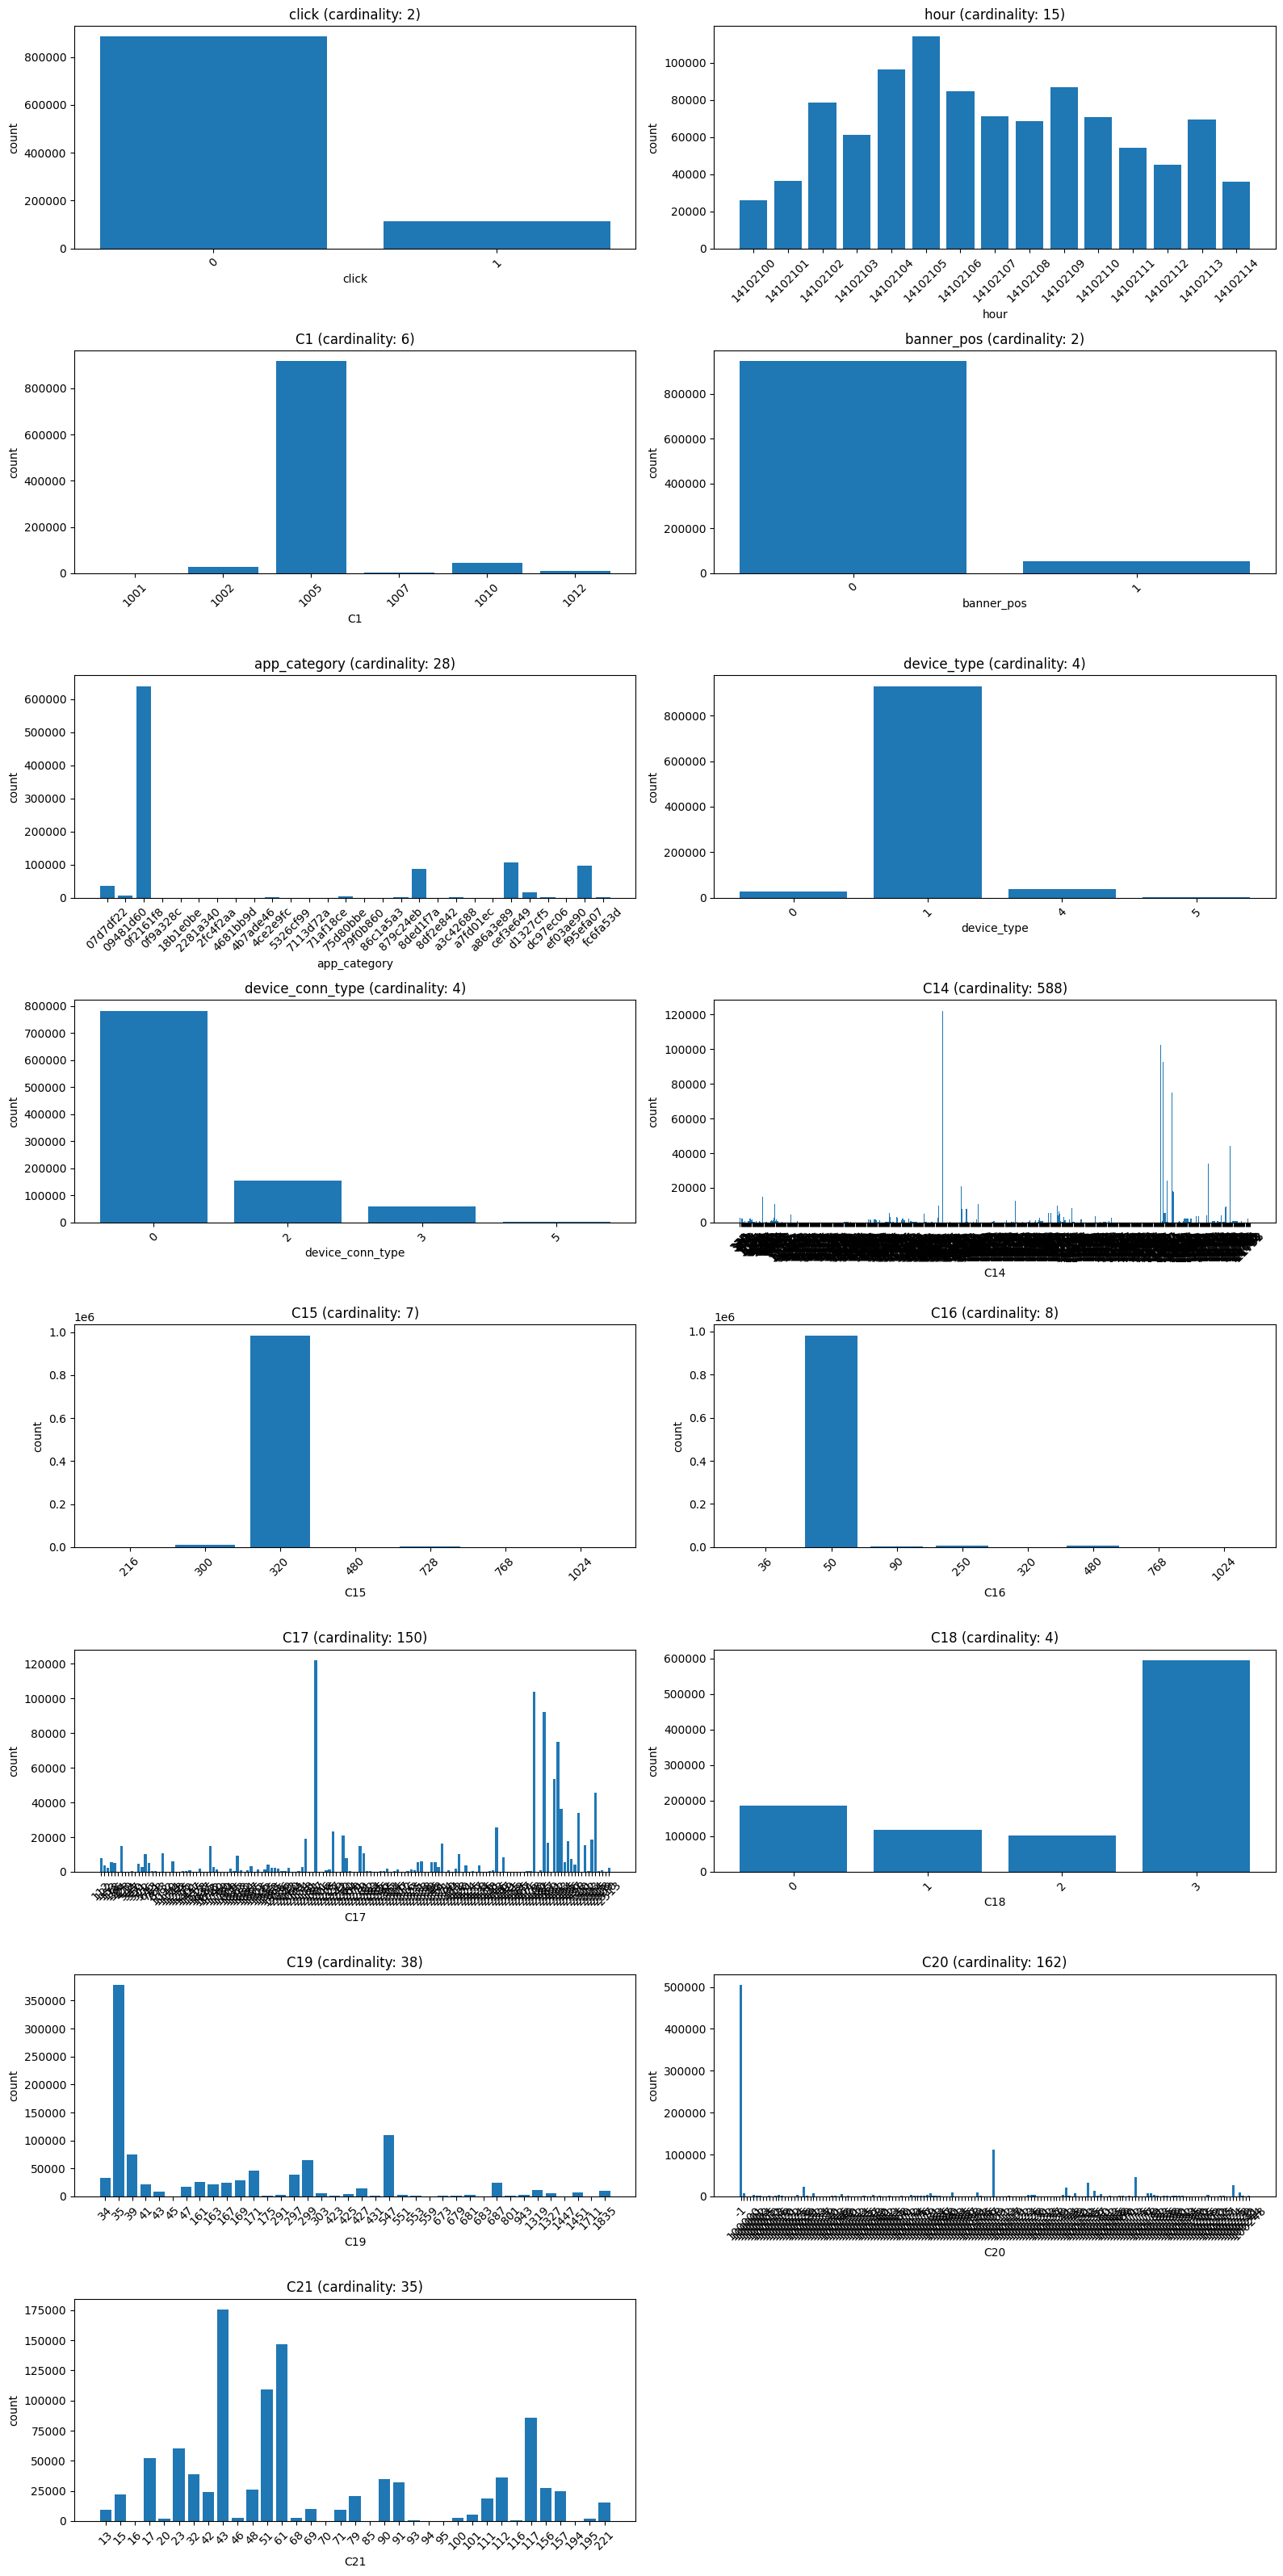
\includegraphics[width=0.65\textwidth]{feature_distribution.png}
\caption{Feature Distributions. Value counts for all retained features, sampled on 1,000,000 impressions. Shows heterogeneity across features.}
\label{fig:features}
\end{figure}

\begin{table}[H]
\centering
\small
\begin{tabular}{llp{6cm}}
\toprule
\textbf{Feature} & \textbf{Type} & \textbf{What It Captures} \\
\midrule
device\_type & Categorical (OHE) & Mobile, tablet, desktop, connected TV --- device context affects ad format suitability \\
device\_conn\_type & Categorical (OHE) & WiFi, 3G, 4G --- connection type affects load behaviour and user intent \\
hour\_of\_day & Numeric (standardised) & Time of day derived from the hour field --- captures temporal patterns in click behaviour \\
app\_category & Categorical (OHE) & Content category of the app --- captures advertised content groupings \\
C1 & Categorical (OHE) & Low-cardinality anonymous categorical feature with meaningful MI signal \\
C20 & Categorical (OHE) & Anonymous categorical feature retained based on MI score \\
C21 & Categorical (OHE) & Anonymous categorical feature retained based on MI score \\
\bottomrule
\end{tabular}
\caption{Context Features for LinUCB. Final context vector is 276-dimensional after one-hot encoding and standardisation.}
\label{tab:context}
\end{table}

\begin{table}[H]
\centering
\small
\begin{tabular}{llll}
\toprule
\textbf{Alpha} & \textbf{Final CTR} & \textbf{Total Regret} & \textbf{Avg Regret} \\
\midrule
0.1 & 0.17379 & 769.13 & 0.00558 \\
0.5 & 0.22159 & 533.76 & 0.00456 \\
1.0 & 0.17125 & 497.15 & 0.00488 \\
1.5 & 0.17182 & 493.63 & 0.00528 \\
\bottomrule
\end{tabular}
\caption{LinUCB Alpha Tuning Results. $\alpha=0.5$ achieves the best CTR and lowest average regret.}
\label{tab:alpha}
\end{table}

\begin{figure}[H]
\centering
\begin{minipage}{0.48\textwidth}
\centering
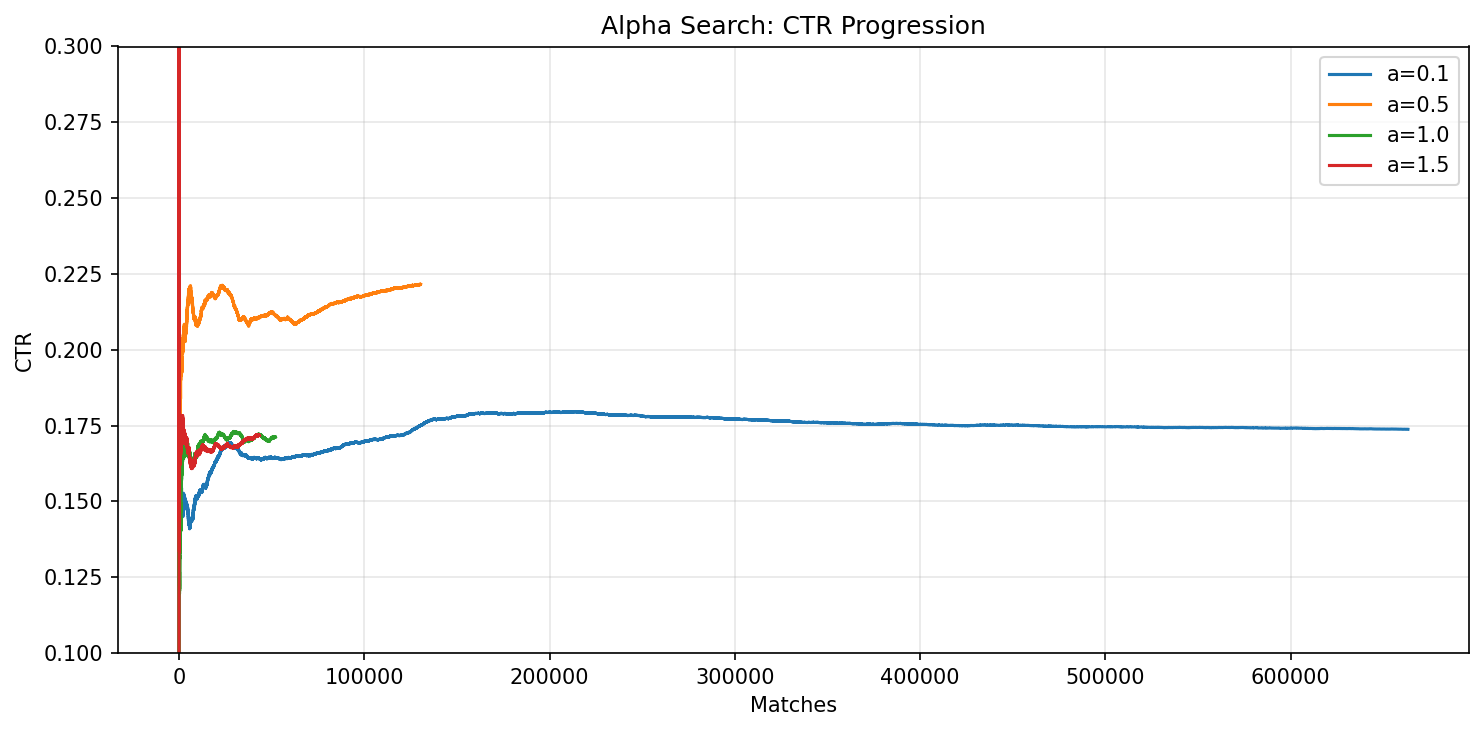
\includegraphics[width=\textwidth]{DBA5113_linucb/plot_alpha_ctr.png}
\caption{CTR Progression}
\label{fig:alpha_ctr}
\end{minipage}
\hfill
\begin{minipage}{0.48\textwidth}
\centering
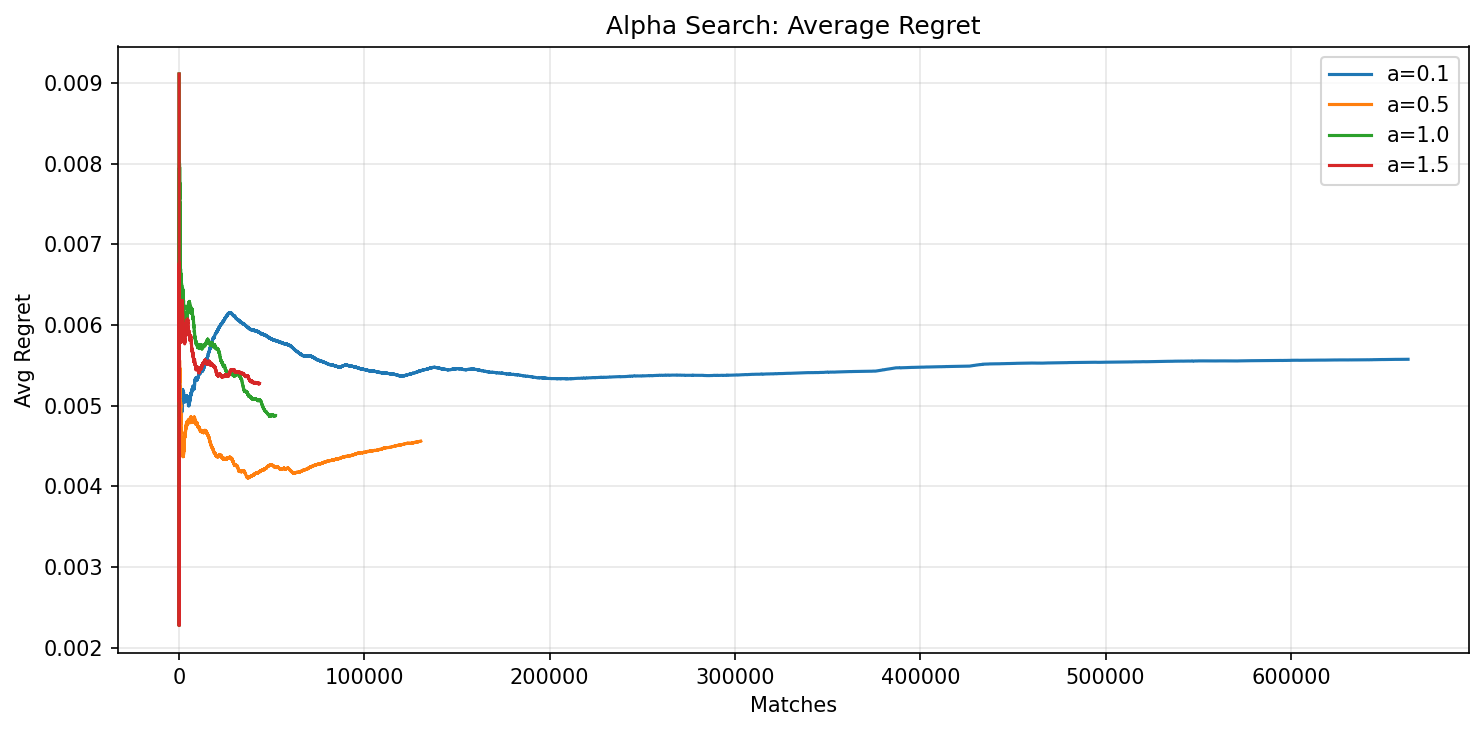
\includegraphics[width=\textwidth]{DBA5113_linucb/plot_alpha_avgregret.png}
\caption{Average Regret}
\label{fig:alpha_regret}
\end{minipage}
\caption*{Alpha Search Results: CTR progression (left) and average regret per impression (right) for candidate $\alpha$ values. $\alpha=0.5$ achieves optimal balance.}
\end{figure}

\begin{figure}[H]
\centering
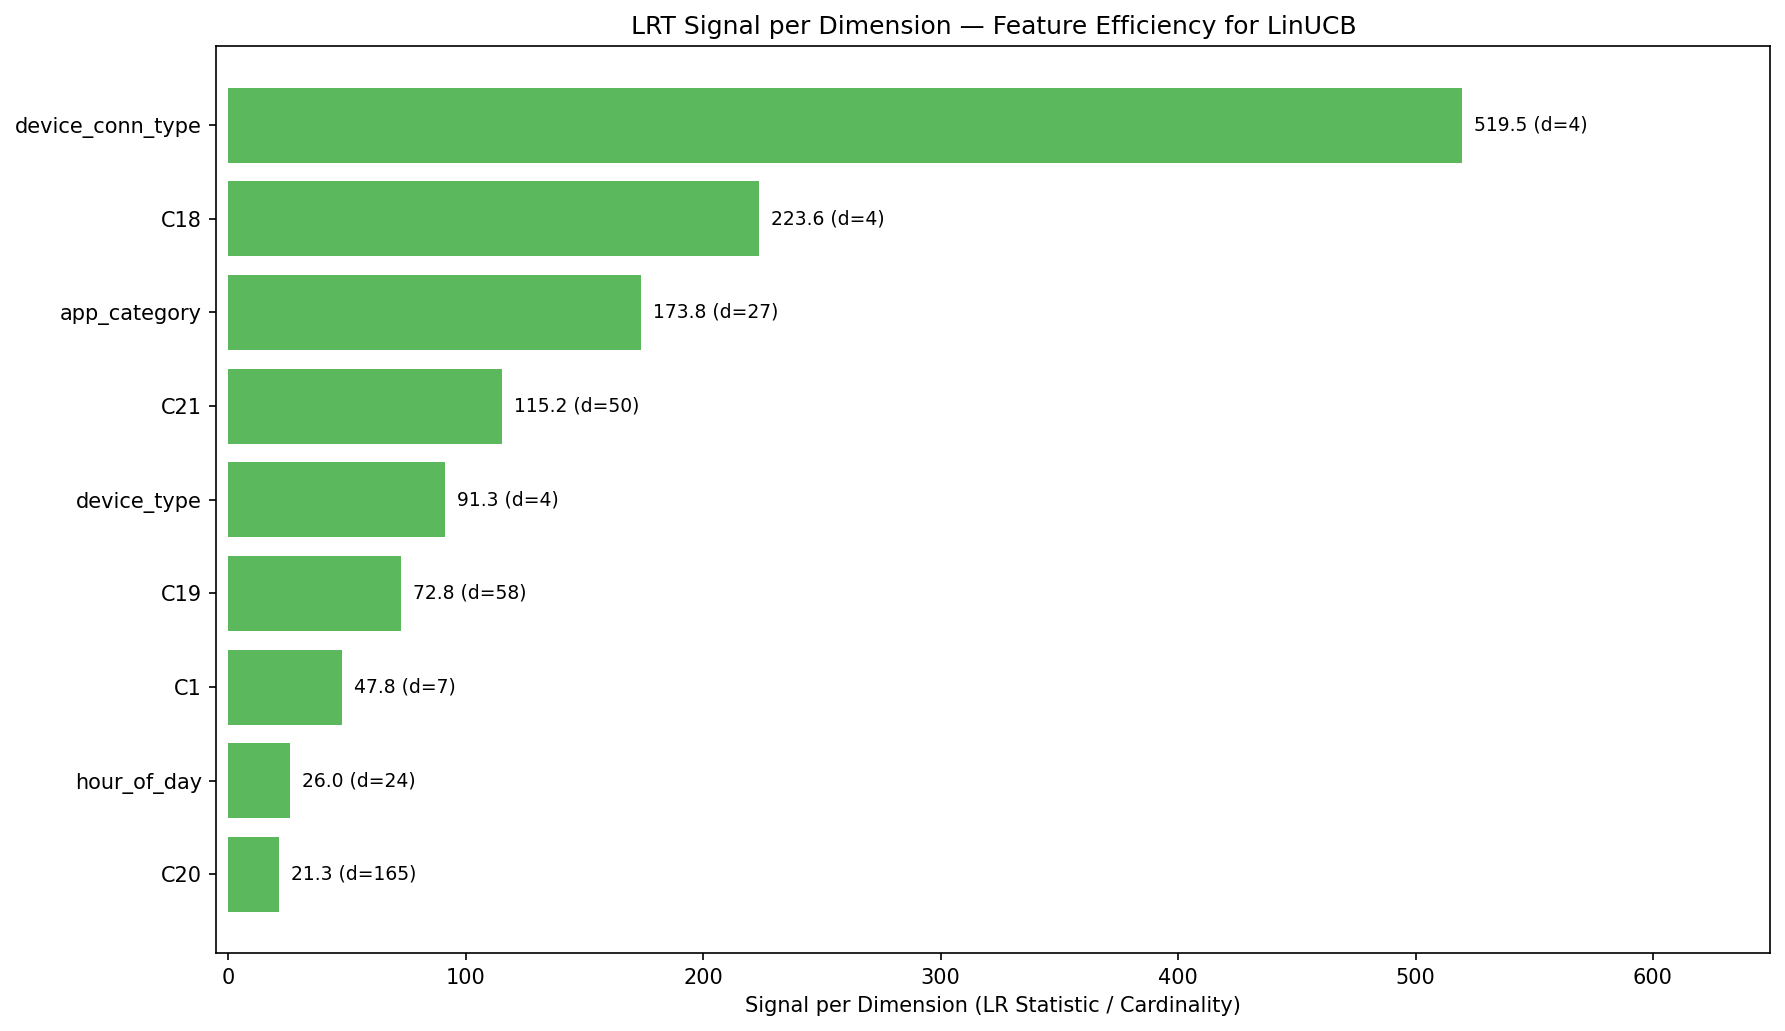
\includegraphics[width=0.7\textwidth]{DBA5113_linucb/lrt_signal_per_dim.png}
\caption{Feature Efficiency: Likelihood Ratio Test Signal per Dimension. device\_conn\_type is far more informative per feature dimension than other features, justifying its prioritisation in context construction.}
\label{fig:lrt_signal}
\end{figure}

\begin{table}[H]
\centering
\small
\begin{tabular}{lllll}
\toprule
\textbf{Algorithm} & \textbf{Type} & \textbf{Final CTR} & \textbf{Avg Regret} & \textbf{Matches} \\
\midrule
Epsilon-Greedy & Non-contextual & 0.13020 & 0.00481 & 1,115,965 \\
UCB & Non-contextual & 0.12852 & 0.00479 & 505,991 \\
LinUCB ($\alpha=0.5$) & Contextual & \textbf{0.22159} & \textbf{0.00456} & 130,409 \\
\bottomrule
\end{tabular}
\caption{Final Algorithm Comparison Metrics. Comprehensive performance metrics for all three algorithms evaluated on the test set.}
\label{tab:final_comparison}
\end{table}

\begin{figure}[H]
\centering
\begin{minipage}{0.48\textwidth}
\centering
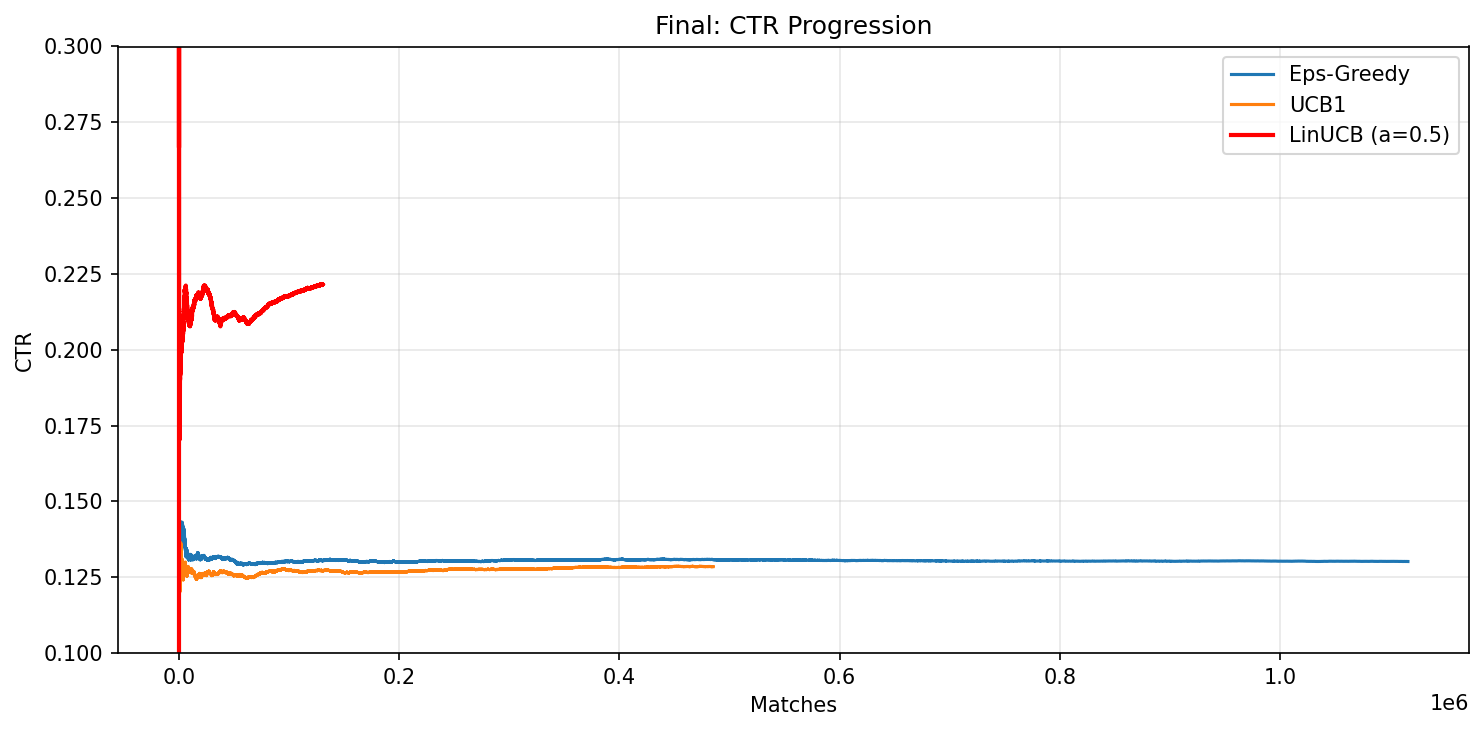
\includegraphics[width=\textwidth]{DBA5113_linucb/plot_final_ctr.png}
\caption{CTR Progression}
\label{fig:final_ctr}
\end{minipage}
\hfill
\begin{minipage}{0.48\textwidth}
\centering
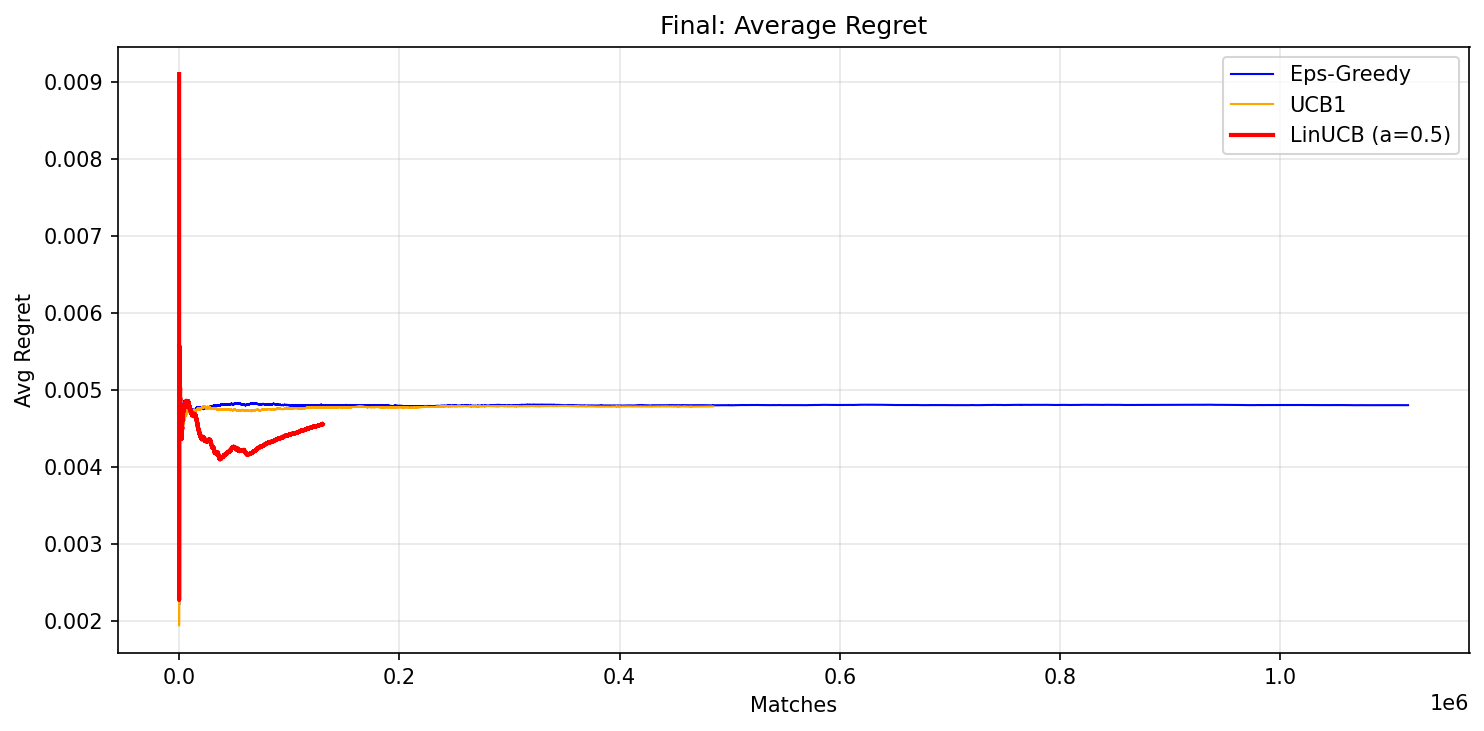
\includegraphics[width=\textwidth]{DBA5113_linucb/plot_final_avgregret.png}
\caption{Average Regret}
\label{fig:final_avgregret}
\end{minipage}
\caption*{Final Algorithm Comparison: CTR progression (left) and average regret per impression (right) across Epsilon-Greedy, UCB, and LinUCB ($\alpha=0.5$). LinUCB achieves substantially higher CTR with lower regret throughout the evaluation period.}
\end{figure}

\begin{figure}[H]
\centering
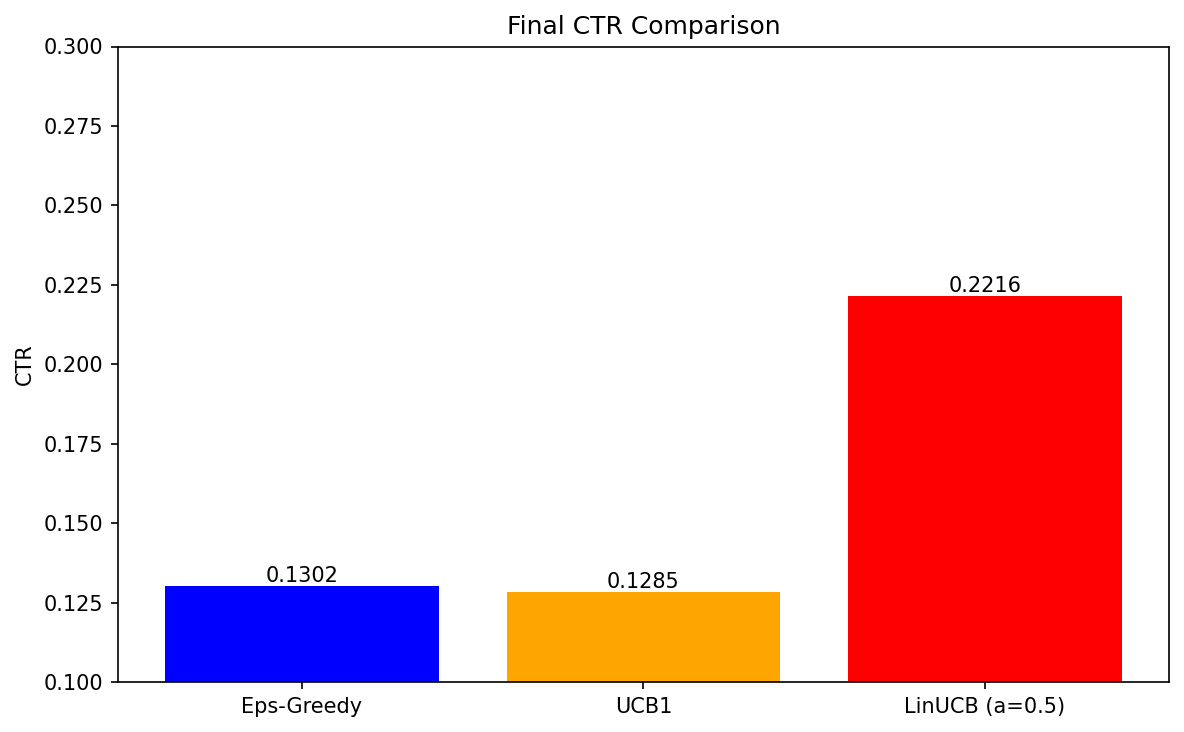
\includegraphics[width=0.6\textwidth]{DBA5113_linucb/plot_final_bar.png}
\caption{Final Performance Comparison: CTR Bar Chart. LinUCB achieves 0.2216 final CTR, representing a 70\% relative improvement over baselines.}
\label{fig:final_bar}
\end{figure}

\end{document}
